
\subsection{Vision}

Die langfristige Vision, die \emph{Flewnit} begleitet, ist die Entwicklung eines interaktiven Paddel-Spiels unter Verwendung dieser Unified Engine mit ausgefeilter Fluid-Mechanik und -Visualisierung, partikelbasierten Rigid Bodies und Dreiecks-Mesh als Repräsentation für statische Kollisions-Geometrie; Spiele, in der große Mengen Fluid, die komplexer simuliert sind als durch Height-Fields
\footnote{s. Kapitel \ref{sec:relatedWork} für mehr Informationen zu Height-Field-basierter Fluidsimulation}
einen integrativen Bestandteil der Spielmechanik ausmachen, sind mir nicht bekannt;\\
Von Dreiecks-Geoemetrie erhoffe ich mir eine genauere Repräsentation zur Kollisionsbehandlung, bei gleichzeitiger Ersparnis vieler Partikel, die sonst z.T große Oberflächen repäsentieren müssten; Ferner könnte die Dreiecksstruktur später zur Simulation nicht-partikelbasierter Rigid Bodies verwendet werden;


\subsection{Paradigmen}
\label{sec:paradigm}

Vor dem Entwurf eines komplexen Softwaresystems mit einigen Zügen, die in etablierten Systemen keine so große Bedeutung haben, hat es Sinn, sich einige Paradigmen zu überlegen, welchen das System nach Möglichkeit folgen soll, um eine gewisse Konsitenz zu gewährleisten:
	
\begin{itemize}
	\item Es wurde beim Entwurf der Unified Engine für jede Simulationsdomäne eine möglichst ähnliche Struktur von Klassen 	
	und ihren Beziehungen zueinander angestrebt. Diese Ähnlichkeit spiegelt sich nach Möglichkeit in einer gemeinsamen 	
	(manchmal abstrakten) Oberklasse eines jeden Konzeptes wider, wie z.B.:
	\begin{itemize}
		\item dem Simulations-Objekt als solchem
		\item der Geometrie
		\item dem Material
		\item der Szenen-Repräsentation
	\end{itemize}
	Auf diese Weise soll eine maximale \emph{Symmetrie} zwischen den Domänen hergestellt werden, so dass domänen-bedingte 
	Spezial-Behandlung von Objekten und Workflows minimiert wird;

	\item Es sollte eine Art Pipeline-Architektur entstehen, wo bestimmte Pipeline-Stages bestimmte Simulations-(Zwischen)-
	Ergebnisse implemetieren, und ggfs. anderen Stages diese zur Verfügung stellen. Jede Simulationsdomäne hat seine eigene 
	Pipeline; Dennoch können Interdependenzen bestehen;\\
	Diesen Interdependenzen wird durch eine Konzept-spezifische Verwaltung durch verschiedene Singleton-Manager-Klassen 	
	genüge getan; Ein und dasselbe Objekt kann von verschiedenen Managern in unterschiedlichem Zusammenhang verwaltet 
	werden; Mehr dazu in Kapitel \ref{sec:systemArchitecture};

	\item Es sollen langfristig so viele Features (Visualisierungstechniken und -effekte, Simulationstechniken) wie möglich 
	miteinander kombinierbar sein, sofern die Kombination nicht unsinnig ist;

	\item Es soll so viel wie möglich auf der GPU berechnet werden, um die massive Paralleltät auszunutzen, 
	und um nicht durch Buffer-Transfers, die die Aufteilung von Algorithmen in CPU- und GPU- Code meist mit sich bringen, 	
	auf den Bandbreiten- und Latenz- Flaschenhals der PCI-Express-Schnittstelle zu stoßen;
	\todo{hier specs und refs zu PCIe 2.0 anbringen? eher nicht, oder?}
	
	\item Es soll immer das Potential gewahrt werden, dass aus dem Framework --- außerhalb des Rahmens dieser 
	Bachelorarbeit --- tatsächlich noch eine Art \emph{Unified Engine} entstehen kann; Somit sind "`schnelle Hacks"',
	also unsaubere Programmier-Weisen, die mit geringstem Programmier-Aufwand ein bestimmtes Feature implementieren,
	überall dort unbedingt zu vermeiden, wo sie die konsistente Gesamstruktur des Systems zu bedrohen scheinen.

\end{itemize}



	


\subsection{Begriffe}

Im Zuge der angestrebten Vereinheitlichung der  verschiedenen Simulation müssen wir auch einige Begriffe verallgemeinern, 
welche in ihrer jahrzentelangen Tradition in der Terminologie der Computergraphik eine spezifische Bedeutung erhalten haben;
Zur besserern Einordnung stellt Abbildung \ref{fig:classicalVsUnified} ein grobes Schema dar, welches die klassische Verwendung verschiedener Engines und die einer Unified Engine gegenüber stellt:



	\begin{figure}[ht]
		%\centering
		\def\svgwidth{\textwidth}
	    \input{classicalVsUnified.pdf_tex}
	   	%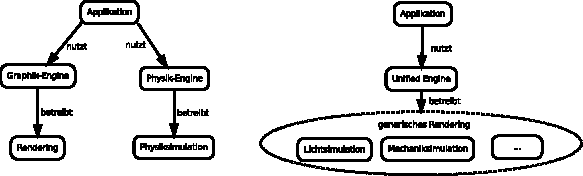
\includegraphics[width=\textwidth]{classicalVsUnified.pdf}
		\caption{Gegenüberstellung von Verwendung und Begrifflichkeiten von klassischen Engines und einer Unified Engine}
		\label{fig:classicalVsUnified}
	\end{figure}
	




\begin{description}

	\item[Rendering]
	Im Wiktionary \cite{internet:wiktionRender} wird das Verb \emph{to render} u.a. umschrieben als:
	\begin{quote}
		"`(transitive, computer graphics) To transform digital information in the form received from a repository into a 
		display on a computer screen, or for other presentation to the user. "'
	\end{quote}	
	Es geht also um die Transformation einer formalen Beschreibung in eine für einen menschlichen Benutzer wahrnehmbare 
	Form. Diese muss entgegen der gewöhnlichen Verwendung des Begriffes nicht zwingend visuell, sondern kann z.B. auch 
	akustischer oder haptischer Natur sein, übertragen durch Lautsprecher oder Force-Feedback-Devices.\\
	
	Verallgemeinern wir den Begriff \emph{Rendering} weiter, gemäß der Übersetzung der Verb-Form als 
	\emph{erbringen}, \emph{machen} \cite{internet:dictCCrender},	
	und in Anlehnung an seine Ethymologie,
	\begin{quote}
		"`From Old French \emph{rendre} (“to render, to make”)"' [...] \cite{internet:wiktionRender}
	\end{quote}
	
	bietet sich eine freie Übersetzung als \emph{Erzeugung eines Zustandes beliebiger Natur} an;\\
	Unter diese generische (Um)-Deutung des Begriffes fällt nun auch \emph{die Ausführung beliebig gearteter Simulation}.
	
	Zu besseren Abgrenzung kann man von \emph{generischen Rendering} und dem klassischen 
	\emph{visuellen Rendering} sprechen; Dies soll im weiteren Verlauf dieser Arbeit der Fall sein.\\
	Eine \emph{Unified Engine} (s.u.) betreibt also \emph{generisches Rendering}.
	
	
	\item[Unified Engine] Alternativ-Bezeichnung: \emph{Unified Rendering Engine};\\
	Eine \emph{Unified Engine} betreibt \emph{generisches Rendering}, indem sie bestimmte Aspekte einer 
	\emph{Welt}\footnote{Diese Welt muss dabei nicht zwingend unserer Realität ähneln oder entsprechen.} simuliert. 
	Darunter kann das klassische (visuelle) Rendering fallen, aber auch die Simulation von Geräuschen und von Mechanik, und 
	beliebige weitere Domänen; Die Domänen sollen dabei durch Abstraktion gemeinsamer Eigenschaften so ähnlich wie möglich
	organisiert sein;
	
	\item[Simulation] Das Begriffspaar \emph{Rendering} und \emph{Physiksimulation} ist im Kontext dieser versuchten 
	Vereinheitlichung nicht mehr angemessen; Stattdessen sollten wir den Simulations-Gedanken aufgreifen und anstelle von
	\emph{Rendering} lieber von \emph{Licht-Simulation} sprechen; Auf diese Weise werden Missverständliche abwechselnde 
	Verwendung vom Begriff \emph{Rendering} vermieden;\\
	Der Begriff der \emph{Physiksimulation} ist auch nicht ganz sauber, da streng genommen Licht auch ein physikalisches
	Phänomen ist, und somit vom Begriff eingeschlossen wird, statt sich abzugrenzen; Es bietet sich die alternative und 
	genauere  Bezeichnung \emph{Mechanik-Simulation} an; Die Quantenmechanik vor Augen (der Name spricht für sich) und 
	damit den Umstand, dass auch Photonen an mechanischen Vorgängen teilnehmen, ist zwar selbst dies keine saubere 	
	Abgrenzung, aber auf dem angestrebten Niveau einer plausiblen (im Kontrast zur "`korrekten"') Echtzeit-Simulation, 
	welche mit der Newton'schen Physik auskommen wird, ist diese Abgrenzung klar genug.
		
	%don't know yet if it makes sense here to define the below words
	%\item[Material] 
	%\item[Buffer] 

	
\end{description}

Somit ist die erste Symmetrie zwischen den Simulationsdomänen durch eine Anpassung der Terminologie bewerkstelligt.





\subsection{Schwerpunkte}

Die Entwicklung eines solchen \emph{Unified Frameworks}\footnote{Von Engine möchte ich Kontext der Implementierung im Rahmen dieser Bachelorarbeit noch nicht sprechen, da dieser Begriff eine viel zu große Vollständigkeit der Implementation suggeriert.} umfasst sehr viele Aspekte, und einige werden wohl in dieser Ausarbeitung keine Erwähnung finden. Um die didaktischen Ziele von Seite \pageref{list:didacticGoals} nicht aus den Augen zu verlieren, wurden folgende Schwerpunkte gesetzt:

	\subsubsection{Entwicklungs-Umgebung}
	Nach Anfängen unter Windows 7 und Visual Studio 2010, gab es bald Probleme beim Compilen von Dependencies auf 
	64 Bit; Womöglich wäre es eine Frage der Geduld gewesen, jedoch habe ich dann zu 
	Ubuntu Linux\footnote{http://www.ubuntu.com/} und Eclipse\footnote{http://www.eclipse.org/} in 
	Kombination mit dem Cross-Platform Build-System CMake\footnote{http://www.cmake.org/} gewechselt. Mir war es sehr 	
	wichtig, ein natives 64-Bit-System zu entwickeln, da viele Register der heutigen 64Bit-Prozessoren sonst ungenutzt 
	bleiben.
	\todo{refernenz finden, bin mir da eher unsicher}
	Das Paket-Management der Linux-basierten Betriebsysteme und die konsequente Implementierung fast aller Programme in 64 
	Bit erleichtern das Einrichten der Dependencies ungemein; Schon alleine dafür hat sich der Umstieg 
	gelohnt.\footnote{Einen sehr sehr großen Dank möchte ich an dieser Stelle Lubosz Sarnecki aussprechen, der mich mit 
	meiner zuvor sehr eingeschränkten Linux-Erfahrung unermüdlich mit Profi-Support bei der fortgeschrittenen Customization 
	des Betriebsystems versorgt hat; Ohne ihn wäre mir dieser schnelle, weitgehend reibungslose Umstieg nicht gelungen.}
	\todo{explizite Danksagung?}

	\subsubsection{Dependencies}
	Das Endziel einer potenten, modernen Engine sollte auf keinen Fall durch die Wahl suboptimaler Bibliotheken 
	eingeschränkt werden; Andererseits sollten, um Compile- und Link-Zeiten gering zu halten und Konflikte zwischen 
	Bibliotheken zu vermeiden, die Dependencies nicht zu komplex sein; Die Wahl vor allem des Fenster-Managers und der
	Mathematik-Bibliothek musste deshalb mit Bedacht getroffen werden; Mehr dazu in Kapitel \label{sec:dependencies}.
	
	\subsubsection{Nutzung moderner OpenGL-Features}
	
	 Uniform Buffers, Tesselation, hardware instancing, verweis auf entpsrechende 
	section;
	
	
	
	\subsubsection{Implemetation und Kombination gängiger visueller Effekte}
	
		-vor allem tesselation, verweise auf entsprechende section
	


	\subsubsection{Buffer-Abstraktion}



	\subsubsection{Template-Engine}
	boilerplate, kombinierbarkeit, nach Möglichkeit lesbarkeit\\
	exemplarischer code schnipsel
		-  Im Zuge des Schwerpunktes auf GPU-Implementierung:
		grantlee gegen boilerplate,zur generierung schlankerer programme als durch Präprozessordierktiven, 
		 $\rightarrow$ einfachere Code- Inspection, verbesserung der lesbarkeit durch generierte, feature-spezifische 	
		 programme,
  		bessere struktur verwaltung des source codees

	\subsubsection{Performance duch Implementierung auf der GPU mit modernen GPU-Computing-APIs}
	auf die massive parallelität eingehen, die sowohl von visualler wie mechanischer domäne genutzt werden kann;
	Performance-Schwerpunkt, Optimierung, auch hardware-abhängige, erwähnen, Gegenüberstellung zu alten OpenGL-nutzenden 	
	GPUPU- Verfahren, die nicht scattern konnten in texturen rendern mussten und auch sonst etliche Nachteile hinnehmen 	
	mussten
	
	
	
	\subsubsection{Effiziente Verwendung von OpenCL}
	 hardware-spezifische bedingte compilings dank grantlee

	\subsubsection{Weiteres}

	 für vielseitig, flexible anwendung zur Laufzeit sollten keine 	Speicher-Lecks auftreten damit Funktionalität 
	 kontrolliert heruntergefahren und neu initialisiert werden kann; 
	 	- memory tracking, (erklären, warum nicht tracking mit Valgrind)
	 
	 Für gemeinsamen zugriff sollten viele Daten für andere Klassen verfügbar sein (Buffer, Rendering Results...); 	
	 Realisierung über Manager-Singleton-Klassen und Zugriff über Map-Container;

	- möglichst hohe Konfiguriertbarkeit ohne ständigen recompile: config file

	
